%%%%%%%%%%%%%%%%%%%%%%%%%%%%%%%%%%%%%%%%%
% ELEE	3720 Electromechanical Energy Conversion: Report template
% By Ratheesh Ravindran
%%%%%%%%%%%%%%%%%%%%%%%%%%%%%%%%%%%%%%%%%
\documentclass[12pt]{article}
\usepackage[english]{babel}
\usepackage[utf8x]{inputenc}
\usepackage{amsmath}
\usepackage{graphicx}
\graphicspath{{images/}}
\usepackage{hyperref}

% Added by me
\usepackage{float}
\usepackage{enumitem}

%\usepackage{fancyhdr}
%\pagestyle{fancy}
\begin{document}
\begin{titlepage}
\newcommand{\HRule}{\rule{\linewidth}{0.1mm}} 
\center % Center everything on the page
 
%---------------------------------------------------------------------------------
%	HEADING SECTIONS
%---------------------------------------------------------------------------------
\textsc{\Large University of Aveiro }\\[0.5cm]
\textsc{\Large Information and Organizational Security }\\[0.5cm]
\textsc{\large Project Assigment }\\[0.5cm]
%---------------------------------------------------------------------------------
%	TITLE SECTION
%---------------------------------------------------------------------------------

\HRule \\[0.4cm]
{ \huge \bfseries Blockchain-based auction management}\\[0.1cm]
\HRule \\[1.5cm]
 
%---------------------------------------------------------------------------------
%	AUTHOR SECTION
%---------------------------------------------------------------------------------



\LARGE \textbf{Authors}\\
\large André \textsc{Pedrosa} 85098 \\
\large Duarte \textsc{Castanho} 85133\\
\vspace{5mm}
\LARGE \textbf{Teachers}\\ 
\large João Paulo Barraca\\
\large Vítor Cunha\\
\vspace{30mm}
{\large \today}\\[1cm]
\vfill

\end{titlepage}

\tableofcontents

%---------------------------------------------------------------------------------
%	DOCUMENT CONTENT
%---------------------------------------------------------------------------------

\newpage

\section{System structure}

\subsection{Clients}
\label{subsec:clients}
The client interaction with the system via command line interface (CLI) has several menus where
  he has to choose an option between a range of numbers. The user's input is always
  checked before, in order to avoid wrong data on the system and crashes \textit{e.g. Make sure the system gets an integer/float for the amount to bet}.\\

In the first approach, we thought about creating the session on the client side, which means that
  the user had to insert their citizen card (CC) only once. As a matter of fact, as every communication
  needed to authenticate the entities, so, we could achieve this by signing data with the private key
  which implies that for every communication we needed the user to insert the PIN code.\\
  This was not the best approach as the user needed to insert the PIN code every time he needed to do some action \textit{e.g. Creating an auction, listing bids, \ldots }


\subsection{Servers}
Both servers possesses a connection endpoint where which clients can exchange requests/responses with it, furthermore 
a server can be a client of another server. \\
As expected each server holds some storage, each one containing only the needed information to execute their designed functions.\\

Both servers are running in Docker containers. When it comes to the Auction Manager, it allow to protect us from the impacts of malicious code, restraining the code's access to the local machine. We decided to Dockerize the Auction Repository as it is a good practice.

\subsubsection{PKI}
As we use hybrid ciphers for entities authentication (\textbf{see section \ref{subsec:handshake}}),
  we need to have asymmetric keys in every entity. As mentioned in \ref{subsec:clients}, clients are
  identified by their CC, but our server don't have nothing to identify them. To solve this problem, we decided to 
  create a set of certificates. \\
Using the application XCA, we created our own Certification Authority (CA), \textbf{SIO CA}, with two
  end entities where both belongs to the two servers, and had their certificates signed
  by our root CA. The CA's certificate was stored locally in all entities. \\
Another way that we could have done, was to distribute the server's certificates, but the
  way we implemented, new services can be added, signed by the CA, plus we don't need to
  get any certificate as we can validate them anyway.
From the XCA application we extracted both certificates and server's private key.
  With the private key being encrypted. plus, at the beginning of the main program of each server, a password
  must be inserted to decrypt it, this simulates an administration password.
Our servers where implemented following a Request Serialization Architecture, which means
  when a connection is made to a server from any client it only processes one process at the time. 
  Every server has a main thread that listens to the connections which every time a connection is received. it
  creates a private socket, sends the information to a Worker thread that handles the process and
  communicates with the client.

\subsubsection{Auction Manager}
Clients and the Auction Repository communicates with the Auction Manager. \\
The former communicates when he wants to:
\begin{itemize}
   \item create an auction or terminate an open one (flow described on \ref{subsec:auctionCreation} 
  and \ref{subsec:auctionTermination}). 
\end{itemize}
  The latter communicates with it when:
\begin{itemize}
  \item  a new bid needs to be validated (item \ref{itm:bidvalidation} of section \ref{sec:newBid} )
  \item when an auction ends after the time defined by the creator (section \ref{subsec:auctionTermination}). \\
\end{itemize}
The manager holds information which is needed to display to the clients, such as the open
  auctions that he can close later, as well associated with an auction, the dynamic code
  to be executed on a bid is validated and the cipher mechanisms to encrypt some fields of
  the bid. \\
It holds two dictionaries:
\begin{itemize}
  \item \textbf{CLIENTS} where the key is the client's id and the value a list of auction created by the clients, which are still open.
  \item \textbf{AUCTIONS} where the key is the auction's id  and the value an Auction class object.
\end{itemize}

The Auction type stores the dynamic code for validation and modification of bids, the base amount
  to bet on that auction, the last amount bet (used by the english auction, Section \ref{subsec:typesOfAuctions}), 
  and the cipher mechanisms to encrypt fields of the bids. These last ones are created 
  for each auction, what means every auction uses different encryption keys, but for all auctions
  we use AES with CBC with PKCS7 padding.

\subsubsection{Auction Repository}
Clients and the Auction manager communicates with the Auction Repository. The former when he
  wants to:
\begin{itemize}
  \item make new bids (section \ref{sec:newBid})
    \item list all open/closed auctions
    \item list all bids sent by a client
    \item list all bids sent to an auction
    \item check the auction's outcome that he participated
    \item validate a receipts (section \ref{sec:receipts})
    \item validate an auction (section \ref{subsec:auctionValidation})
\end{itemize}
The latter communicates with it when:
\begin{itemize} 
  \item a new auction is created
  \item when the auction's creator wants to close an auction. \\
\end{itemize}
For each client, the repository holds information about what auction he participated in order to display
  the bids that he made (in case of hidden identities only the bids from closed auctions are shown).
  For the auctions, each one has one blockchain and all operation over an auction, such as getting all
  the bids, making a new bid, \ldots, are done by querying/manipulating the block. \\
It holds three dictionaries:
\begin{itemize}
  \item \textbf{CLIENTS} where the key is the clientId of each client and the value a set containing
    the id of the auctions that a client participated
  \item \textbf{CLIENT\_BIDS\_COUNT} where the key is the clientId and the value is another dictionary where its keys are auctionId, and the value is
  the number of bids made to that auction.
  \item \textbf{OPEN\_AUCTIONS} where the key is  the auction's id and the value an Auction class object
  \item \textbf{CLOSED\_AUCTIONS} where the key is the auction's id and the value an Auction class object
\end{itemize}

The auction type has an BlockChain class object. This BlockChain class is a linked list
    of Block class objects and it holds a reference to the first (where the auction
    information is stored) and last block (to insert new blocks more easily).\\ 
    The Block type has:
  \begin{itemize}
    \item a block number 
    \item the hash of the previous block
    \item a nonce, some data (dictionary)
    \item the block's hash (pre-calculated) 
    \item a reference to the next block.
  \end{itemize}

\section{Communication}

For the communication between the entities we used \textbf{Transmission Control Protocol} (TCP).

\subsection{Messages}
Every message that we send is a JSON object. \\
Our messages can be in clear text or encrypted. Clear text messages are only sent during
  the establishment of a secure connection between entities (more detail on section \ref{subsec:handshake}).
  Beyond that, all messages are encrypted. \\
A clear text message can have a pre defined structure but depends on which step the handshake is in. 
  The encrypted messages always have 3 fields, an iv/nonce, the ciphertext and a mac.

\subsection{Encryption}
To make our messages unique the entities must send a messageId. This field is calculated with
  \[sessionId + sequenceNumber\] where \textit{sessionId} is a random byte string of 32 bytes and \textit{sequenceNumber}
  is the order of the message, e.g for the first message an encrypted message is create with
  \[E(\{"messageId":sessionId+sequeceNumber, "someField":\dots\}, someKey)\]. \\

\subsubsection{Asymmetric}
\begin{figure}[h]
  \center{
    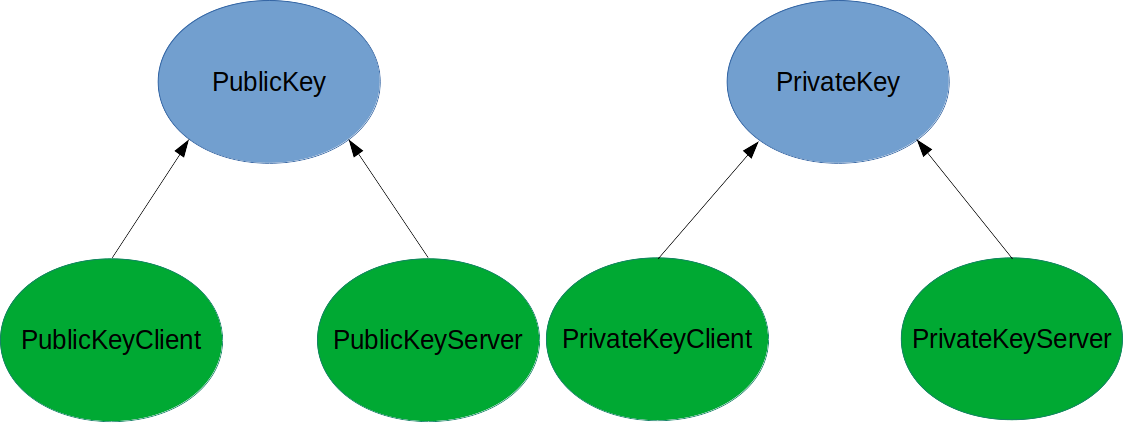
\includegraphics[scale=0.30]{asymmetric.png}
  }
  \caption{Class diagram of asymmetric keys (Blues are abstractions)}
  \label{fig:asymmetric}
\end{figure}
Both clients and servers need asymmetric keys, but they have different types of
  backends. The clients uses the CC and the servers their keys directly.
  That would lead making different codes when using one or another. So to prevent that
  we created the abstraction tree  represented in \textit{figure \ref{fig:asymmetric}}. \\
There are two types of keys, private and public, each one has two types, one for the user, 
  in case of the private key interacts with the CC, and one for the servers. \\

  \begin{itemize}
  \item A server public key can encrypt and verify signatures. 
  \item A user public key can only verify signatures. 
  \item A server private key can sign data and decrypt data. 
  \item A user private key it only can sign. 
  \end{itemize} 

In terms of mechanisms for the user, we sign data with PKCS1v15 padding and for the servers, after reading
  the cryptography package documentation they recommended using PSS padding so we did that.
  As the CC only accepts encryption with SHA1 and SHA256 hash algorithms, we chose  SHA256.

\subsubsection{Symmetric}
\begin{figure}[h]
  \center{
    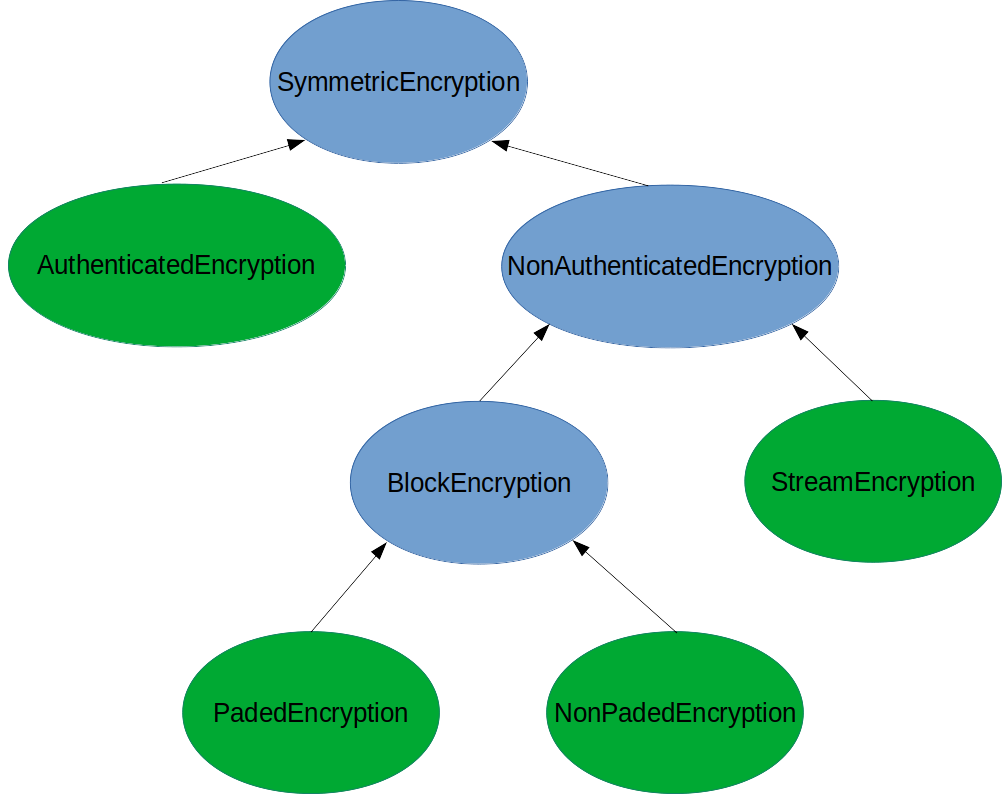
\includegraphics[scale=0.25]{symmetric.png}
  }
  \caption{Class diagram of symmetric encryption possibilities (Blues are abstractions)}
  \label{fig:symmetric}
\end{figure}
For symmetric encryption exists a wide combination of possibilities for what mechanisms can be used such as AES with CBD, ChaCha20, AESGCM, \ldots \\
To allow all the combinations we built the tree of classes represented in the \textit{figure \ref{fig:symmetric}}. All
  the classes have a cipher and a key. Then we can have some mechanisms with built-in integrity control
  and others who don't. The ones that have the mac field on the messages is an empty string. For those that
  don't have built-in integrity control we use hash-based message authentication codes (HMAC) with SHA256 as hash algorithm. \\ 
Within the non authenticated encryption we can have stream cipher (ChaCha20) and block ciphers. 
  The block cipher may or may not need padding as some modes transform a block cipher into a stream cipher.

\subsection{Handshake}
\label{subsec:handshake}
\begin{figure}[h]
  \center{
    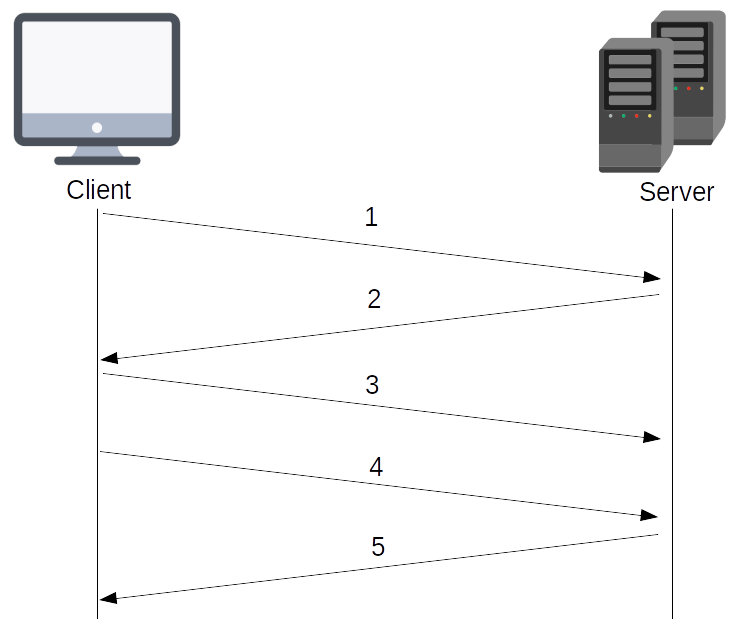
\includegraphics[scale=0.35]{handshake.png}
  }
  \caption{Flow of interactions between a client and a server when doing and handshake}
  \label{fig:handshake}
\end{figure}
Before any connection a secure tunnel needs to be established authenticating both entities, 
  and exchanging cryptographic information to be used later in the connection. 
  Our handshake was based on the Transport Layers Security (TLS). 
  The flow of interactions is shown on the \textit{figure \ref{fig:handshake}}. We wrote client but a client can 
  be a server as a server may want to communicate with other server, e.g. when a clients
  creates an auction the auction manager has to communicate with the auction repository.
\begin{enumerate}[label=\textbf{\arabic*}]
  \item \textbf{Client - Supported cipher mechanisms} \\
    The client sends the cipher mechanisms to the server but he must send three lists for supported cipher algorithms, 
      supported modes, and supported padding algorithms. To choose what mechanisms to consider we
      read the documentation of the cryptography package and there was some information for some modes or
      algorithms that were improper to use in some cases or weak, \textit{e.g. mode ECB (weak) and
      mode XTS (meant to disk encryption)}. \\ 
    We don't negotiate hash algorithms as some certificates
      were sign with different hash algorithms so we assume that everybody supports all of them.\\
      On the client main we do a random over the possible
      mechanisms to represent the system's heterogeneity. Furthermore, the servers support all the mechanisms.

  \item \textbf{Server - Chosen mechanisms, certificate, authentication data}
    From the mechanisms received  the server chooses the best ones. It gives priority to cipher algorithms with
      built-in authenticating, then to stream cipher, then to block cipher that don't need padding and 
      finally to padded block ciphers. Basically it goes from top to bottom over the tree on the 
      \textit{figure \ref{fig:symmetric}}. \\
    It sends the chosen cipher, mode and padding algorithms, sends his certificate and a random byte string 
      of 64 bytes to later authentication of the client.

  \item \textbf{Client - Certificate verification, shared keys} \\
    The clients validates the certificate received by checking if it expired, if it was
      revoked by checking the locally store CRL's and if it's an end-entity where the key usage must 
      be to digital signatures only. If all went well it builds the trust chain by getting the issuer 
      of each certificate until a certificate self signed (\(issuer == subject \)). For each of this 
      certificates it checks if it is expired and if it was revoked on the moment when he signed the 
      other certificate and is also checked the key usage that must be to sign certificate only. Now, 
      if all went well, it is checked if the signatures in the chain is valid by checking if a signature
      of a certificate was signed by the issuer mentioned. \\ 
    The user also creates the 2 to 3 random byte string. One for the symmetric encryption (size depends 
      on the chosen cipher mechanism), another for the sessionId (32 bytes) and a third one for the
      integrity control in case the chosen cipher mechanism doesn't have built-in authentication of data. 
      This keys are encrypted with the public key of the server extracted form his certificate received. \\
    The user also signs the authentication data received with his private key.

  \item \textbf{Client - Handshake finish} \\
    The user sends a encrypted message with the field "finished handshake".

  \item \textbf{Server - Handshake finish} \\
    After the verification is complete as is item 3 and if all went well, it sends a encrypted message with the field 
      "finished handshake".
\end{enumerate}

\section{Bids}
\label{sec:newBid}
\begin{figure}[h]
  \center{
    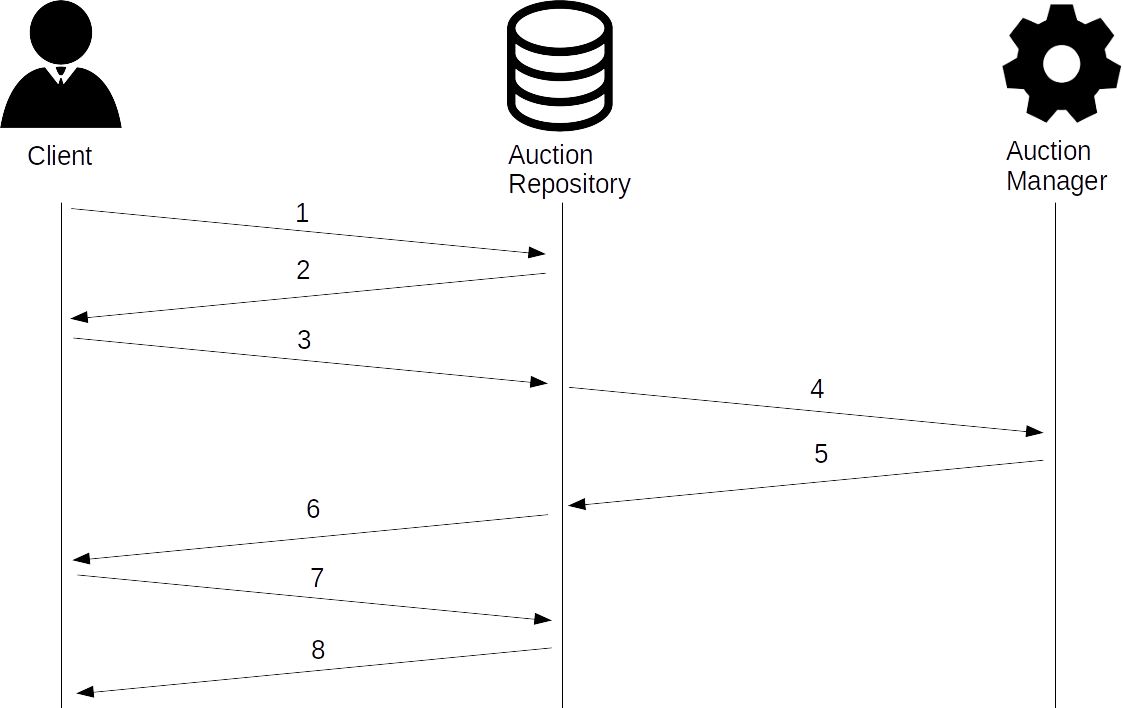
\includegraphics[scale=0.35]{newBid.png}
  }
  \caption{Flow of communications on the system to make a new bid}
  \label{fig:newBid}
\end{figure}

To explain everything about what Security mechanisms are being used on the bids we go over the process
  for creating a new bid and explain what we used. The whole process is illustrated on the \textit{figure
  \ref{fig:newBid}}

\begin{figure}[h]
  \center{
    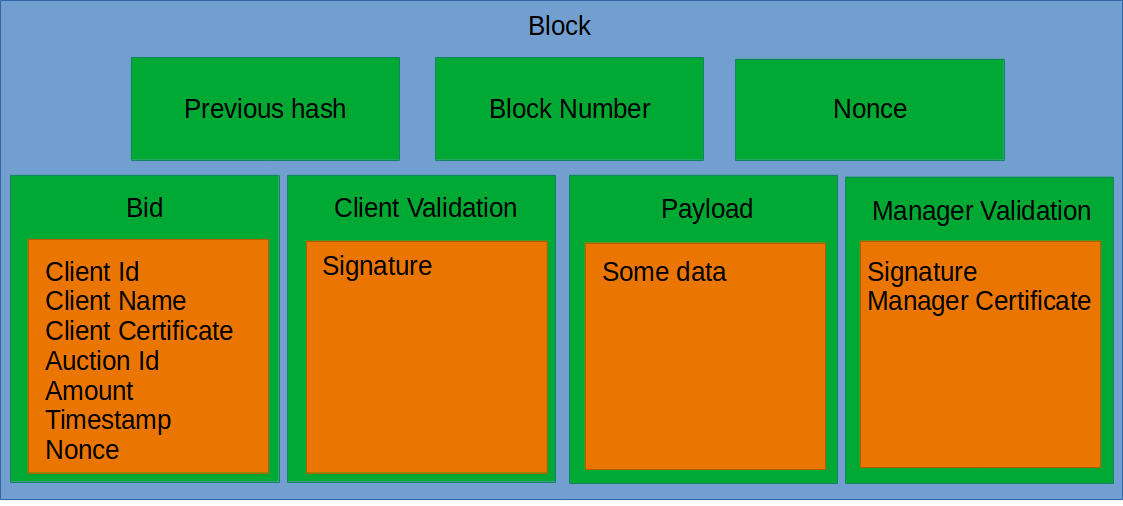
\includegraphics[scale=0.35]{block.png}
  }
  \caption{Content of a block of the blockchain}
  \label{fig:block}
\end{figure}

The process of making a new bid is basically inserting a new block on the blockchain with the data associated
  with the bid. On the \textit{figure \ref{fig:block}} is the complete structure of a block for a new bid.

\begin{enumerate}
    \item Client - requests for the information of all open auctions that he can make bids

    \item Repository - sends the requested information

    \item Client - chooses the auction and sends the information needed to construct the bid on the 
      \textit{figure \ref{fig:block}} (timestamp, auction Id, nonce and amount. The client name, client id, 
      and the certificate of the client is the repository that can obtain from the handshake). The nonce
      field is to make the bid unique so attackers can't discover fields of the bid by brute forcing
      for example the signature mentioned next. Although he just sends some of the field, locally he constructs the 
      bids, makes an hash of it (SHA256) and signs it. This signature is the client validation field of the block

    \item Repository - after checking if the signature is ok, sends the data received (Bid and clients validation)
      to the manager.

    \item Manager - Here the manager encrypts the necessary fields if the auction's type says that. 
    \label{itm:bidvalidation}
      If the identities have to be hidden then the Manager encrypts all the fields including the client validation except the 
      bid's amount. If the type of the auction said that the amount needs to be hidden then just the 
      amount is encrypted. The nonce is always encrypted. \\
      After that comes the bid's validation. This can be achieved by doing through dynamic code. 

      If the validation accepts the bid the manager runs the modification code created by the owner 
        of the auctions. This code has as objective to add something more to the block that the auction 
        creator may want to add. This new data will go into the payload field of the block.
      After all this, the manager signs the content that he created by doing a hash over the bid (with 
        encrypted fields), the client validation (can be encrypted) and the payload. Finally the manager 
        adds a new field to the blocks data, manager validation, with his certificate and the signature 
        mentioned before.

    \item Repository - one of the problem of the auctions is that several people can make bids at the same
      \label{itm:cryptopuzzle}
      time very quickly. This can be controlled by using a mechanism called cryptopuzzle. This is a task that 
      is hard to perform and very easy to verify if it is right. Our cryptopuzzle implementation was 
      based on the BitCoins cryptopuzzle where the hash of the new block as to be inferior of a certain 
      value. This value can adjusted to make easier or harder to make new bids. This field is defined 
      by the user on the auction creation. Because we are using SHA256 for the hashing the value of 
      an hash can go from 0 to \(2^{256}\). We can allow adjustments of the difficulty in the formula
      \[2^{256-d}\]
      where d is a value in the interval \([0,256[\). The higher the d, the hard it is to make new bids.
      The repository adds to the block's data the \(number of the previous block + 1\) and the hash of the 
      previous block.

    \item Client - What the user has to do is to generate a random nonce and keep trying until the hash 
      of the block is under the specified value. When it is sends the hash and nonce found to the repository.

    \item Repository - The repository verifies the solution presented by the client by just doing a hash
      over the blocks data with the nonce sent by the client. If it is under the target and is equal to
      what the client calculated the bid is accepted and adds a new block to the block chain with the 
      information that was hashed (\textit{figure \ref{fig:block}}). Also if the auction has identities publicly 
      available, it inserts the auction's ID to the set of client's participated auctions that made the bid.\\
      If the new bid was completed successfully, it returns the receipt of that bid. This receipt serves to prove that
      the bid was added to the auction. 

\end{enumerate}

\section{Auctions}
\subsection{Types of Auctions}
\label{subsec:typesOfAuctions}
\begin{itemize}
    \item English \\
      Identities are hidden and amount of the bids are publicly available
    \item Bling with identities shown \\
      Amount of the bids are hidden and identities are publicly available
    \item Bling with identities hidden \\
      Identities and amount of the bids are hidden
\end{itemize}

\subsection{Creation}
\label{subsec:auctionCreation}

See \textit{figure \ref{fig:auctionCreation}}.

\begin{figure}[h]
  \center{
    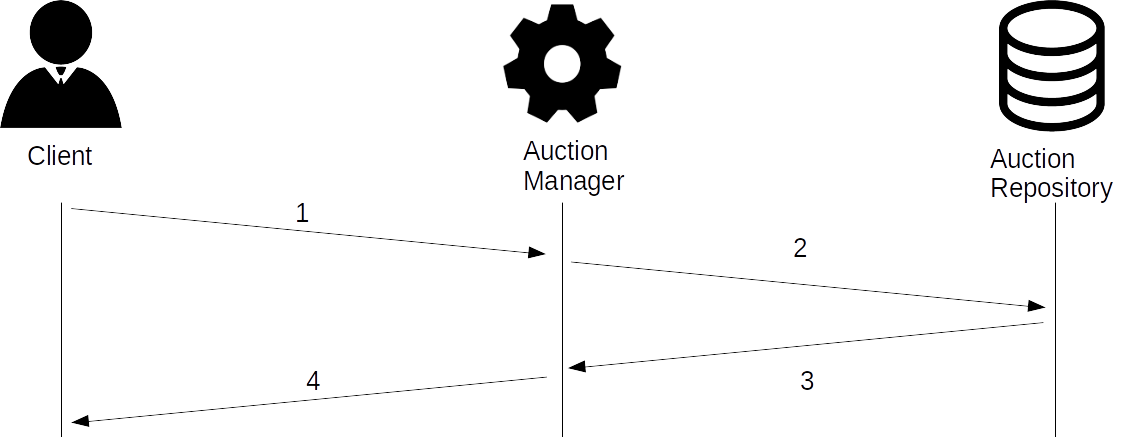
\includegraphics[scale=0.35]{auctionCreation.png}
  }
  \caption{Flow of communications on the system to create an auction}
  \label{fig:auctionCreation}
\end{figure}

\begin{enumerate}
  \item Auction Information \\
    The clients sends all the information needed to create an auction:
    \begin{itemize}
      \item Type
      \item Name (max 40 characters)
      \item Description (max 200 characters)
      \item Duration (in minutes)
      \item Difficulty (in the interval \([0,256[\). See section \ref{itm:cryptopuzzle} of section
         \ref{sec:newBid})
      \item Base amount
      \item Validation code
      \item Modification code
    \end{itemize}
    
    In the validation code, the user has the control to manipulate the validBid variable and has also access to data that its content
    depend on the auction type.

    \begin{itemize}
      \item English Auction - Access to \textit{amount} and \textit{lastAmount} variables.
      \item Blind Shown - Access tp \textit{clientId}, \textit{clientName}, \textit{clientCertificate}, \textit{countBidsDone} and \textit{timestamp} 
      variables
      \item Blind Hidden - It has access to none variables  
    \end{itemize}


  \item Instantiation on the repository \\
    The auction Manager does a syntactic validation and if it is nothing wrong, instantiates a new auction on the auction repository by sending all the 
      information received adding:
    \begin{itemize}
      \item Creator name
      \item Creator ID
    \end{itemize}
    both extracted from the CC.

  \item Save to storage (Repository) \\
    The repository adds to the auction information
    \begin{itemize}
      \item Creation time
      \item Auction Id
    \end{itemize}
    The auction repository creates an Auction object and places it on the OPEN\_AUCTIONS dictionary
      associating to the auctionId. Then it mines the first block (calculates the hash) where the block number 
      is 0, the previous hash and nonce is a 32 byte string of zeros and the data is the information of the 
      auction. Also, starts a timer thread that executes, after the duration defined by the creator, it
      terminates the auction. Finally adds the creator's participated auctions list the auction
      created so he can later see the outcome of the auction.

  \item Save to storage (Manager) \\
    The manager receives from the repository the auctionId and the creation time of the auction created
      and saves it to the AUCTIONS dictionary associating to the auctionId. When a auction creation occurs, a new key is randomly generated and the auctionID it is added to the list of the user's open auctions.
    
\end{enumerate}

\subsection{Termination}
An auction can be closed for two reason. Because the creator sends that order to the manager 
  (\textit{figure \ref{fig:auctionTermination}}) or because the duration defined to the auction as come to the end 
  (\textit{figure \ref{fig:auctionTerminationTime}}).

\label{subsec:auctionTermination}

\begin{figure}[h]
  \center{
    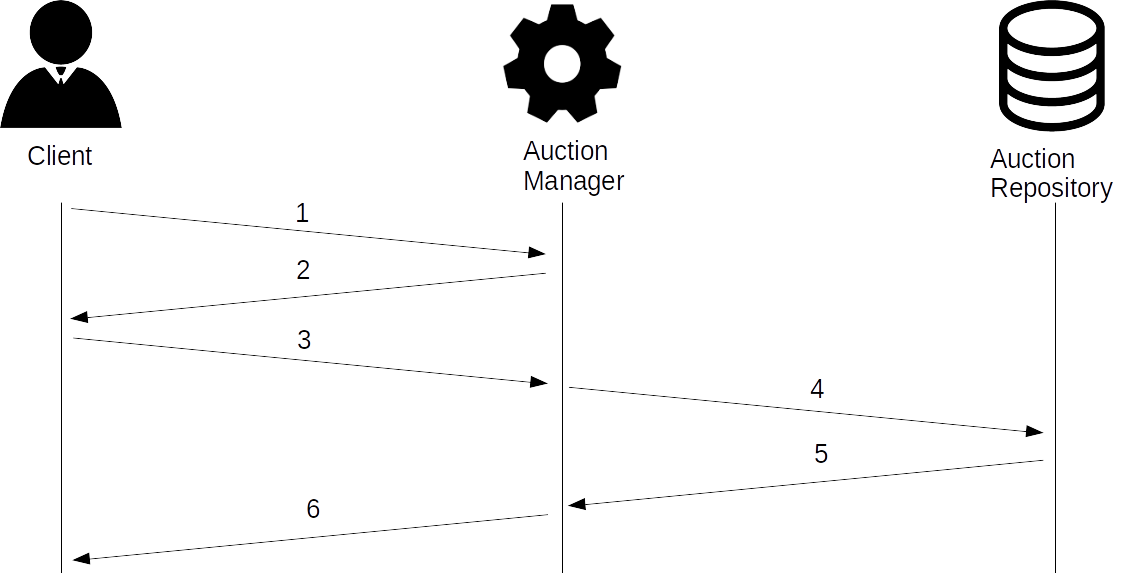
\includegraphics[scale=0.35]{auctionTermination.png}
  }
  \caption{Flow of communications on the system to terminate an auction}
  \label{fig:auctionTermination}
\end{figure}

For the first case:

\begin{enumerate}
    \item The clients asks the manager for the information of all the auctions
      that he created and that are still open

    \item The manager sends the information requested

    \item The clients chooses the auction he wants to close and sends the auction id

    \item The manager sends to the repository the key used to encrypt the fields
      for that auction so he can calculate the winner. Another option was to the manager 
      request all the bids, and them he calculate the winner and send again. We considered
      this approach because the repository receives much more request than the manager but
      this implies to send all the bids through the network what can be slow.

    \item The repository calculates the winner of the auction and creates a last block with
      a nonce of 32 bytes of zeros, and the data is the block's number where the winner bid is plus the key received. 
      The repository sends the winner bid to the manager to latter display to 
      the creator. \\
      Also moves the auction from the OPEN\_AUCTIONS to the CLOSED\_AUCTIONS and stops the timer
        thread.

    \item The manager propagates the message received to the client and deletes the information
      of the auction that was closed and removes the auctionId from the list of open auction of the 
      client.

    \item The clients receives the winner bid and sees how much many the auction has brought him.

\end{enumerate}

\begin{figure}[h]
  \center{
    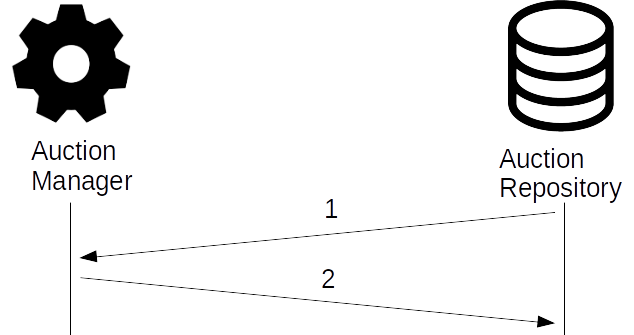
\includegraphics[scale=0.35]{auctionTerminationTime.png}
  }
  \caption{Flow of communications on the system when the time of an auction ends}
  \label{fig:auctionTerminationTime}
\end{figure}

For the case where the duration of the auction ends there is a timer thread that is responsible
  to make the necessary actions to close the auction. As there are multi threading involved
  we have a semaphore with starting state of 1 that a thread needs to acquire before doing anything
  on the storage of the repository.

\begin{enumerate}
    \item The repository asks for the key that he used to encrypt the fields of the
      bids for that auction.
    \item The manager sends the requested information deleting the information
      of the auction that was closed and removes the auctionId from the list of open auction of the 
      client. \\
      The repository does the same as described on the step 5 of \textit{figure \ref{fig:auctionTermination}} 
      except sending of the winner bid to the manager.

\end{enumerate}

\subsection{Validation}
\label{subsec:auctionValidation}



\begin{figure}[h]
  \center{
    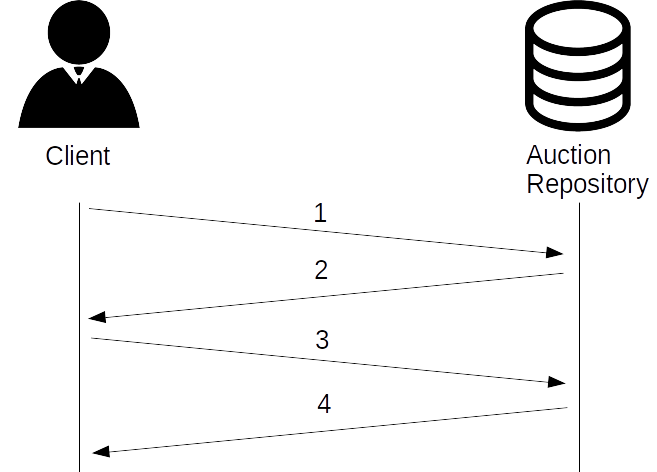
\includegraphics[scale=0.35]{./images/validateAuction.png}
  }
  \caption{Flow of communications on the system when a clients wants to validate an auction}
  \label{fig:auctionValidation}
\end{figure}

\begin{enumerate}
    \item Client - asks information of all the auction to choose one
    \item Repository - sends the information requested
    \item Client - chooses the auction and sends the auction id to the repository
    \item Repository - sends the information every block on the blockchain of that auction \\
      The clients verifies the last block. If it has the block's number where is located the winner bid and the key that
      was used to cipher the fields of the bids then he can validate all the signatures, hashes 
      that were created during the creation of the every bid (section \ref{sec:newBid}). Can validate:
      \begin{itemize}
        \item the chain of blocks has a sequence of valid hashes (validated through previous hashes)
        \item validate the signature of the manager of the payload and encrypted bid
        \item validate the signature of the client over the decrypted bid
      \end{itemize}
      However if the auction didn't finish yet, the client can only validate:
      \begin{itemize}
        \item the chain of blocks that has a sequence of valid hashes (validated through previous hashes)
        \item the manager's signature of the payload and encrypted bid
      \end{itemize}

\end{enumerate}
\vspace{20mm}

\section{Receipts}
\label{sec:receipts}

The receipt is a prove that a client receives to ensure that he made a new bid, previously explained 
  in \textit{figure \ref{fig:newBid}}. The client guarantees that he will, for each bid added to an auction, 
  the Client stores its receipt in  memory for later validation, towards preventing both servers from cheating by manipulating the sequence of bids in an auction.
\vspace{30mm}

Programmatically speaking it is a list of all block's content. In another words, the entire BlockChain.  

\subsection{Receipt Validation}
\label{subsec:receiptValidation}

\begin{figure}[h]
  \center{
    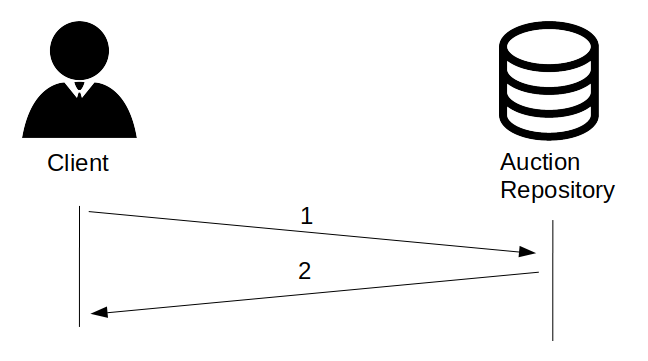
\includegraphics[scale=0.35]{validateReceipt.png}
  }
  \caption{Flow of communications on the system when client validates receipt}
  \label{fig:validateReceipt}

  \begin{enumerate}
    \item Client - asks the auction's data to validate the receipt
    \item Repository - returns the auction's data 

\end{enumerate}
\end{figure}


\end{document}
